% Supplementary material of main.tex — generic template (plain article class). To move to a venue class
% (IEEEtran, acmart, llncs, ...), keep the body and replace the preamble and the front matter.
% Build:  latexmk -pdf main.tex
% Figures: figures/paper_figures.ipynb (style: figures/paper_style.py; dataset_construction.py runs on the server)
% Notes for the authors would be in \todo{...} (red). The previous draft is in _da_cancellare/.
\documentclass[11pt,a4paper]{article}
\usepackage[margin=2.5cm]{geometry}
\usepackage[T1]{fontenc}
\usepackage[utf8]{inputenc}
\usepackage{lmodern}
\usepackage{amsmath,amssymb}
\usepackage{graphicx}
\usepackage{booktabs}
\usepackage{xcolor}
\usepackage{tikz}
\usetikzlibrary{arrows.meta,positioning,shapes.misc}
\usepackage[numbers,sort&compress]{natbib}
\usepackage{xr-hyper}
\usepackage[colorlinks=true,linkcolor=blue!50!black,citecolor=blue!50!black,urlcolor=blue!50!black]{hyperref}
\def\UrlBreaks{\do\/\do-\do\_\do.}
\usepackage{authblk}
\usepackage{orcidlink}
\renewcommand\Affilfont{\small}

\externaldocument[M-]{main}
\newcommand{\todo}[1]{\textcolor{red}{[\textbf{TODO:} #1]}}
\newcommand{\anon}{\operatorname{anon}}

\renewcommand{\thesection}{S\arabic{section}}
\renewcommand{\thetable}{S\arabic{table}}
\renewcommand{\thefigure}{S\arabic{figure}}

\title{Supplementary material for ``Reading the Source: Predicting the Reliability of Unseen News Publishers from the
Anonymized Text of Their Articles''}
\author{}
\date{}

\begin{document}
\maketitle

\section{The anonymization in detail}\label{app:anonfig}
Figure~\ref{fig:anonymization} shows what each pass of the anonymization of Section~\ref{M-sec:anon} replaces.

\begin{figure}[t]
\centering
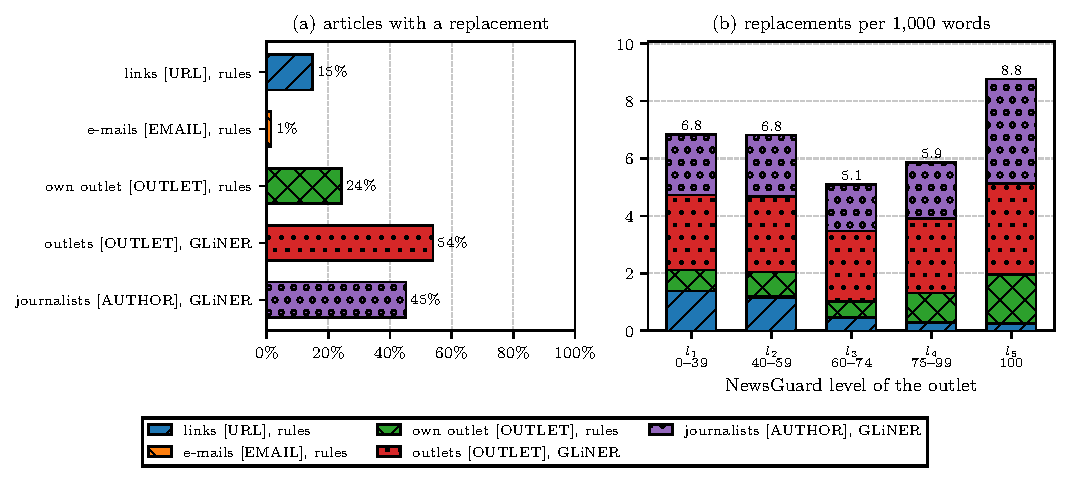
\includegraphics[width=\linewidth]{figures/anonymization.pdf}
\caption{The anonymization of the 25,524 articles. (a) Share of articles with at least one replacement of each kind
(passes 1--2: links, e-mail addresses, the outlet's own name; pass 3, GLiNER: other outlets and journalists). (b)
Articles whose title or text still contains the name of their own outlet. (c) Replacements per 1,000 words by
NewsGuard score band of the outlet (mean over articles).}\label{fig:anonymization}
\end{figure}


\section{More metrics}\label{app:measures}
Table~\ref{tab:more} adds three metrics to Table~\ref{M-tab:main}, on the same outlets, predictions and resamples: the
coefficient of determination $R^2$ (the share of the variance of the NewsGuard score explained by the predictions), the
root mean squared error, which weighs large errors more than the MAE, and the area under the ROC curve for telling the
reliable outlets (score $\geq 60$, NewsGuard's threshold; 65\% of the outlets) from the others. The AUC uses only the
order of the predictions, so it is not affected by their compression. The order of the models is the same as with the MAE for $R^2$ and the RMSE. On the binary distinction, however, the large frozen models are only slightly ahead of TF-IDF (0.876 and 0.880
against 0.860): their advantage lies more in how close the predicted score is to the rating than in which side of 60 an
outlet falls on.

\begin{table}[h]
\centering
\caption{More metrics per outlet (226 outlets, all articles), with 95\% bootstrap intervals.}\label{tab:more}
\resizebox{\linewidth}{!}{%
\begin{tabular}{lccc}
\toprule
model & $R^2$ & RMSE (points) & AUC, score $\geq 60$ \\
\midrule
no text (training mean) & 0.000 [$-$0.023, 0.000] & 27.0 [24.8, 29.3] & 0.501 [0.422, 0.577] \\
no text (training median) & $-$0.058 [$-$0.130, $-$0.013] & 27.8 [25.1, 30.5] & 0.500 [0.500, 0.500] \\
orientation only & 0.223 [0.101, 0.327] & 23.8 [21.3, 26.5] & 0.688 [0.611, 0.762] \\
Mistral-Small-24B-Instruct, zero-shot & $-$0.085 [$-$0.261, 0.031] & 28.2 [26.3, 30.0] & 0.665 [0.589, 0.738] \\
\midrule
TF-IDF + ridge & 0.339 [0.273, 0.392] & 22.0 [20.1, 24.0] & 0.860 [0.807, 0.907] \\
ModernBERT (fine-tuned) & 0.341 [0.253, 0.415] & 22.0 [19.9, 24.0] & 0.835 [0.781, 0.884] \\
ModernBERT (frozen) + ridge & 0.308 [0.236, 0.365] & 22.5 [20.6, 24.5] & 0.824 [0.769, 0.875] \\
Qwen3-Embedding-0.6B (frozen) + ridge & 0.268 [0.209, 0.316] & 23.1 [21.1, 25.1] & 0.838 [0.782, 0.891] \\
Qwen3-Embedding-8B (frozen) + ridge & 0.437 [0.368, 0.496] & 20.3 [18.4, 22.2] & 0.880 [0.831, 0.923] \\
Mistral-Small-24B (frozen) + ridge & 0.475 [0.406, 0.533] & 19.6 [17.7, 21.5] & 0.876 [0.827, 0.920] \\
\bottomrule
\end{tabular}}
\end{table}

\section{Other splits of the outlets}\label{app:splits}
The results of Table~\ref{M-tab:main} come from a single split of the outlets into five folds. To see how much they
depend on it, we repeated the three ridge models with four more splits, made with the same procedure (folds stratified
on the exact score) and different random seeds; everything else is as in Section~\ref{M-sec:setup}
(Table~\ref{tab:splits}). The models are ranked in the same order in every split, on both metrics. Mistral-Small-24B
lowers the error of TF-IDF by 2.0--2.3 points in every split (2.2 on average) and raises $\rho$ by 0.03--0.07;
Qwen3-Embedding-8B lowers it by 1.5--1.9 points and raises $\rho$ by 0.01--0.04. The error of each model varies by
less than half a point across splits, and the split of the paper is the one where Mistral-Small-24B lowers the error of
TF-IDF least.

\begin{table}[h]
\centering
\caption{The three ridge models with five splits of the outlets (the first is the split of the paper): MAE and
Spearman $\rho$ per outlet, all articles.}\label{tab:splits}
\small\setlength{\tabcolsep}{4pt}
\begin{tabular}{lcccccc}
\toprule
& \multicolumn{2}{c}{TF-IDF} & \multicolumn{2}{c}{Qwen3-Embedding-8B} & \multicolumn{2}{c}{Mistral-Small-24B} \\
\cmidrule(lr){2-3}\cmidrule(lr){4-5}\cmidrule(lr){6-7}
split seed & MAE & $\rho$ & MAE & $\rho$ & MAE & $\rho$ \\
\midrule
1 (paper) & 17.8 & 0.674 & 16.3 & 0.711 & 15.8 & 0.735 \\
2 & 17.9 & 0.690 & 16.3 & 0.696 & 15.7 & 0.720 \\
3 & 18.2 & 0.660 & 16.5 & 0.688 & 16.0 & 0.716 \\
4 & 18.0 & 0.673 & 16.1 & 0.713 & 15.8 & 0.742 \\
5 & 18.2 & 0.673 & 16.5 & 0.692 & 16.1 & 0.722 \\
\midrule
mean (SD) & 18.0 (0.17) & 0.674 (0.010) & 16.3 (0.15) & 0.700 (0.011) & 15.8 (0.17) & 0.727 (0.011) \\
\bottomrule
\end{tabular}
\end{table}

\section{Robustness checks}\label{app:robust}
Table~\ref{tab:robust} reports three checks on the MAE of Table~\ref{M-tab:main}, on the same predictions; in
parentheses the difference from TF-IDF in the same row. \emph{Recalibrated}: the outlet scores re-mapped by a straight
line fitted, in every outer fold, on the training outlets only, with predictions from three inner folds (for the
zero-shot model, on its answers for the training outlets); it removes most of the compression, lowers every error, and
leaves Mistral-Small-24B better than TF-IDF ($-1.5$ [$-2.7$, $-0.4$]) but not Qwen3-Embedding-8B ($-0.9$ [$-2.0$,
0.2]). \emph{Re-weighted}: the MAE per NewsGuard level weighted by the share of each level among the political outlets
that could not be collected (43\% in the lowest level, against 15\% in the dataset) or among all the political outlets
sent to the scraper: the error to expect on a population of unrated outlets is about 20 points for Mistral-Small-24B.
\emph{Without the 16 outlets} whose brand name, as recorded by NewsGuard, is still in the anonymized text of at least one
article.

\begin{table}[h]
\centering\small
\caption{MAE per outlet under three checks (in parentheses: difference from TF-IDF).}\label{tab:robust}
\resizebox{\linewidth}{!}{%
\begin{tabular}{lccccc}
\toprule
& TF-IDF & Qwen3-Embedding-8B & Mistral-Small-24B & zero-shot & no text (median) \\
\midrule
as in Table~\ref{M-tab:main} & 17.8 & 16.3 ($-$1.5) & 15.8 ($-$2.0) & 24.4 (+6.6) & 22.1 \\
recalibrated inside the training folds & 16.2 & 15.3 ($-$0.9) & 14.7 ($-$1.5) & 21.2 (+5.0) & -- \\
re-weighted: outlets not collected & 22.9 & 20.9 ($-$2.0) & 20.2 ($-$2.7) & 22.8 ($-$0.1) & 34.9 (+12.0) \\
re-weighted: all political outlets & 22.4 & 20.4 ($-$2.0) & 19.7 ($-$2.7) & 24.0 (+1.6) & 32.6 (+10.1) \\
without the 16 outlets with their brand name & 18.0 & 16.5 ($-$1.4) & 16.2 ($-$1.8) & 24.4 (+6.5) & -- \\
\bottomrule
\end{tabular}}
\end{table}

\section{An earlier, rule-based anonymization}\label{app:anon}
Before the anonymization of Section~\ref{M-sec:anon}, we ran the whole pipeline, including the fine-tuned ModernBERT, with
a simpler anonymization made of six rules: the outlet's signature in the titles, e-mail addresses, links, social media
accounts, the outlet's own authors taken from the author field of the page, and the outlet's name. Unlike the
recognizer, these rules mask only the publisher and its own staff. Table~\ref{tab:anon} compares the two anonymizations
on the same outlets and articles. Masking every outlet and journalist changes the language models by at most 0.010 in
$\rho$ and 0.24 points of error, never significantly with all articles; only TF-IDF loses a little ($\Delta\rho =
-0.017$ [$-0.036$, $-0.001$]), consistently with a model that uses names of outlets and people as features. With 1, 5
and all articles per outlet and the four metrics of Table~\ref{M-tab:main}, 8 of the 12 comparisons of TF-IDF are worse
with the stricter anonymization (95\% bootstrap interval of the difference excluding zero, no correction), against 3
of 12 for Mistral-Small-24B and none for the other two models.

\begin{table}[h]
\centering
\caption{Spearman $\rho$ and MAE per outlet with the six-rule anonymization of the first run and with the
anonymization of the paper (all articles).}\label{tab:anon}
\begin{tabular}{lcccc}
\toprule
& \multicolumn{2}{c}{six rules} & \multicolumn{2}{c}{rules + GLiNER} \\
\cmidrule(lr){2-3}\cmidrule(lr){4-5}
model & $\rho$ & MAE & $\rho$ & MAE \\
\midrule
TF-IDF & 0.691 & 17.7 & 0.674 & 17.8 \\
Qwen3-Embedding-8B & 0.722 & 16.1 & 0.711 & 16.3 \\
Mistral-Small-24B & 0.735 & 15.7 & 0.735 & 15.8 \\
ModernBERT & 0.605 & 17.7 & 0.610 & 17.5 \\
\bottomrule
\end{tabular}
\end{table}

\section{Who is left out by the cleaning}\label{app:selection}
Table~\ref{tab:selection} describes the 1,293 political outlets sent to the scraper by the step at which they left the
dataset. The outlets that could not be collected and those removed with the duplicates are much less reliable than
those in the dataset, and the second group is almost entirely made of the network of 164 copies of
Section~\ref{M-sec:groups}.

\begin{table}[h]
\centering
\caption{The political outlets by the step at which they left the dataset: number, mean NewsGuard score, share in each
level, share by orientation and share based in the United States (\%).}\label{tab:selection}
\resizebox{\linewidth}{!}{%
\begin{tabular}{lrrrrrrrrrrr}
\toprule
removed at & outlets & score & $l_1$ & $l_2$ & $l_3$ & $l_4$ & $l_5$ & left & right & none & US \\
\midrule
no article collected & 619 & 41.4 & 43 & 35 & 5 & 13 & 3 & 7 & 50 & 43 & 68 \\
text extraction & 6 & 78.2 & 0 & 33 & 0 & 50 & 17 & 0 & 67 & 33 & 50 \\
English & 91 & 73.6 & 11 & 14 & 9 & 45 & 21 & 20 & 22 & 58 & 15 \\
100--1,500 words & 12 & 55.0 & 25 & 17 & 25 & 25 & 8 & 8 & 67 & 25 & 67 \\
published from 2025 & 34 & 56.4 & 21 & 41 & 6 & 24 & 9 & 29 & 26 & 44 & 76 \\
exact duplicates & 170 & 37.0 & 89 & 2 & 2 & 6 & 1 & 7 & 5 & 88 & 98 \\
near duplicates & 14 & 27.9 & 93 & 0 & 7 & 0 & 0 & 0 & 29 & 71 & 100 \\
at least 10 articles & 60 & 57.5 & 22 & 35 & 10 & 25 & 8 & 27 & 35 & 38 & 77 \\
one outlet per group & 61 & 47.8 & 13 & 69 & 7 & 10 & 2 & 36 & 59 & 5 & 97 \\
\textbf{in the dataset} & 226 & 68.5 & 15 & 19 & 13 & 35 & 17 & 30 & 44 & 26 & 79 \\
\bottomrule
\end{tabular}}
\end{table}

\section{The zero-shot prompt}\label{app:prompt}
The system message and the user message given to Mistral-Small-24B-Instruct, through its chat template:

\begin{quote}\small
You are an expert media analyst. NewsGuard rates news and information websites with a score from 0 to 100, the weighted sum of nine journalistic criteria: the site does not repeatedly publish false content (22 points), gathers and presents information responsibly (18), regularly corrects or clarifies errors (12.5), handles the difference between news and opinion responsibly (12.5), avoids deceptive headlines (10), discloses ownership and financing (7.5), clearly labels advertising (7.5), reveals who is in charge, including possible conflicts of interest (5), and provides the names of content creators with contact or biographical information (5). Scores below 60 mean that the site generally fails to meet basic standards of credibility and transparency.

\smallskip\noindent Below is one article published by a news website. The names of news outlets have been replaced by \texttt{[OUTLET]}, the names of journalists by \texttt{[AUTHOR]}, links by \texttt{[URL]} and e-mail addresses by \texttt{[EMAIL]}.

\smallskip\noindent Estimate the NewsGuard score (0-100) of the website that published this article. Answer with a single integer and nothing else.

\smallskip\noindent Article:
\emph{<the anonymized article>}
\end{quote}

\section{What else was tried on these outlets}\label{app:tried}
The rules of the dataset, the split and the models of the paper were fixed in earlier rounds of experiments on the same
226 outlets, whose test results we saw. We list them so that the comparisons can be read accordingly; the ridge penalty
and the Mistral layer are the only choices made inside the training folds.
\begin{itemize}
  \item Classification of the five NewsGuard levels instead of regression of the score, with TF-IDF, the frozen models
        and ModernBERT.
  \item Other models: Gemma-27B as a frozen encoder, dropped because its half-precision outputs overflowed on our GPU;
        layer 40 of Mistral-Small-24B, now chosen on the inner folds; DeBERTa as a fine-tuned encoder, in an earlier round
        on the exact score with three splits of the outlets. The hyper-parameters of ModernBERT (5 epochs, learning rate
        $3 \cdot 10^{-5}$) come from an earlier round on these outlets.
  \item Fourteen other regressors on the frozen vectors of Qwen3-Embedding-8B and Mistral-Small-24B: kernel ridge, a
        small neural network, attention over the articles of an outlet, models at the outlet level, weights for outlets
        and rare scores, mixup. In that analysis no method was much better than the ridge (the best, the small neural
        network, lowered the error of Mistral-Small-24B by about one point), and the advantage over TF-IDF did not depend
        on the regressor.
  \item Predictions re-mapped to the quantiles of the training scores, which lower the MAE, and outlets represented by
        groups of their articles.
  \item The rule-based anonymization of Section~\ref{app:anon}.
\end{itemize}
The stability of the results over five splits of the outlets (Section~\ref{app:splits}) limits how much these choices
can have adapted to the folds.

\section{Released resources and the demonstration tool}\label{app:tool}
\begin{table}[t]
\centering\small
\caption{Resources released with the paper. Nothing released contains NewsGuard scores, NewsGuard levels or article
text. \emph{Study}: \url{https://github.com/bianchi-john/PublisherClassification}; \emph{tool}:
\url{https://github.com/bianchi-john/publisher-evaluation}.}\label{tab:release}
\begin{tabular}{p{0.15\linewidth}p{0.50\linewidth}p{0.11\linewidth}p{0.12\linewidth}}
\toprule
resource & content & repository & licence \\
\midrule
pipeline code & every step of Sections~\ref{M-sec:data}--\ref{M-sec:experiments}: scraping, cleaning, anonymization,
  split, models, evaluation, tables and figures & study & Apache-2.0 \\
models & the four main models of Table~\ref{M-tab:main} (TF-IDF, Qwen3-Embedding-8B, Mistral-Small-24B,
  fine-tuned ModernBERT), each in its five fold versions (one per held-out fold of outlets):
  TF-IDF and the ridge heads as arrays, ModernBERT as ONNX & tool & Apache-2.0 \\
predictions & for each of the 25,524 articles: id, URL, outlet domain, fold and the out-of-fold score of the four
  models & tool & CC BY 4.0 \\
split & the 226 outlet domains and their fold & tool & CC BY 4.0 \\
tool & \emph{Publisher Evaluation}: scores new articles with the released models (below) & tool & Apache-2.0 \\
\bottomrule
\end{tabular}
\end{table}

The released models derive from base models distributed under the Apache-2.0 licence: the fine-tuned encoder from
ModernBERT-base, and the two frozen representations from Qwen3-Embedding-8B and Mistral-Small-24B-Base-2501, whose
weights are not redistributed but downloaded from Hugging Face by the tool. The anonymization uses the large
GLiNER model of Section~\ref{M-sec:anon} (Apache-2.0), also downloaded on first use.

\paragraph{The tool.}
\emph{Publisher Evaluation} runs on the user's machine, with a web interface and a command line
(Figure~\ref{fig:tool}). Given a URL or a pasted text with the domain of its outlet, it extracts the text as in
Section~\ref{M-sec:cleaning} and refuses what is outside the training data rather than extrapolating: pages that are not
a single article, texts that are not in English or not between 100 and 1,500 words. A pasted text gets an identifier
that marks it as given by the user, so that it is never mistaken for a downloaded page. The tool then anonymizes the
text with the procedure of Section~\ref{M-sec:anon} and shows it with the placeholders highlighted and the list of the
names the recognizer replaced, so that the user sees exactly what the models read. The user chooses which of the
available models to run; each predicts the score of the outlet from this one article, and the score of an outlet is
the mean over its stored articles, with the standard deviation and a bootstrap interval of this mean, which describe
the spread of the article predictions, not the error of the outlet score (about 16 points on average,
Table~\ref{M-tab:main}). The released predictions are
loaded from the start, so the 226 outlets of the paper can be browsed, compared across models and exported, and a
page lists the models found on disk with their status (ready, missing a GPU, invalid with the reason). Every number is
presented as a model prediction, not as a rating: one article is a weak signal (Section~\ref{M-sec:stage1}). The tool
can also be started in a read-only public mode, which shows the released data and evaluates nothing.

\begin{figure}[t]
\centering
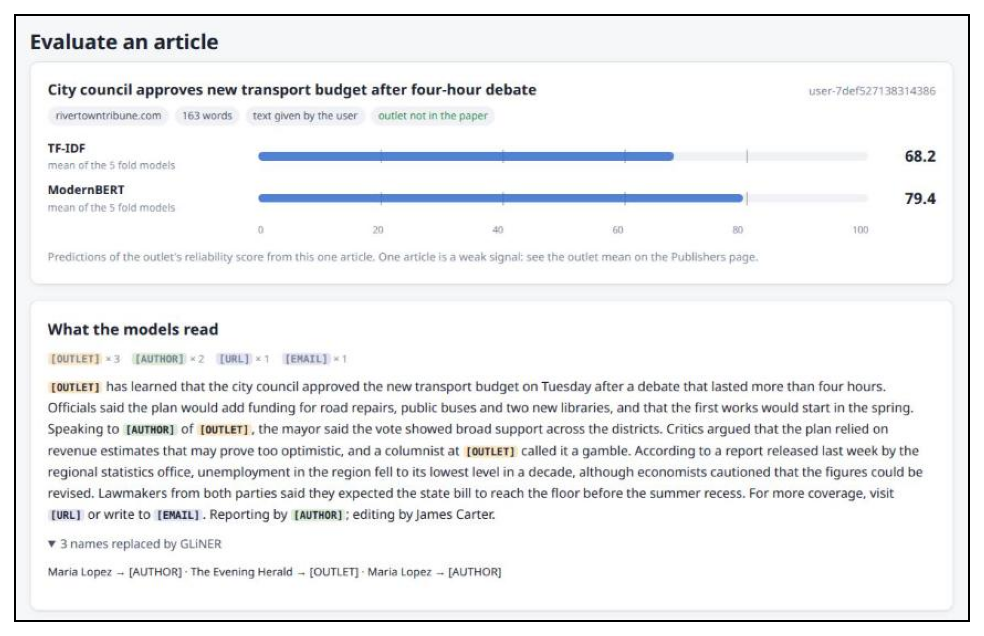
\includegraphics[width=0.92\linewidth]{figures/tool.pdf}
\caption{The Evaluate page of \emph{Publisher Evaluation}, on an invented test article (not a real outlet) and with
the two models that run on a CPU (the frozen language models need a GPU). Top: the predicted score of the outlet from
this article, for each model; the outlet is new, so each score is the mean of the five fold models. Bottom: the text
the models read, with the placeholders of the anonymization highlighted and the names replaced by the recognizer.}
\label{fig:tool}
\end{figure}

\paragraph{Models and fidelity.}
The models are shipped in formats that execute no code from the model files: TF-IDF and the ridge heads as plain
arrays, rebuilt by the tool, and ModernBERT as an ONNX graph in half precision, as in our experiments. Against the
paper's predictions, the TF-IDF scores are identical and the ridge heads differ by less than $10^{-4}$ points on all
the articles, and ModernBERT by 0.05 points on average (at most 1 point) on 1,500 checked articles; the anonymization
of the tool reproduces that of the paper exactly on a sample of 40 articles. Qwen3-Embedding-8B and Mistral-Small-24B
are downloaded once from Hugging Face and need a GPU (about 18 GB); without one, TF-IDF and ModernBERT score new
articles on a CPU (about 1 s per article and fold for ModernBERT) and the released predictions of all four models
remain available.

\paragraph{Leakage guard.}
The model of fold $k$ was trained on the outlets of the other four folds. For an article of one of the 226 outlets, the
tool uses only the model of the fold that held that outlet out, so that no outlet is scored by a model that saw it in
training; for a new outlet, the score is the mean of the five fold models. An article of the paper that is evaluated
again keeps its id and is never counted twice.

\paragraph{Custom models.}
Users can add their own regressors of the 0--100 score as ONNX graphs, reading either the anonymized text or its
tokens. A custom model is used only after strict checks: a valid graph with only the operators built into ONNX and
onnxruntime, exactly the declared inputs and a single score output, and a probe run on 20 synthetic anonymized articles
(finite scores within the scale, not all equal, the same when scored again and when scored in a batch). Its manifest
declares which outlets it was trained on, and the same leakage guard applies (a model that declares nothing is never
used on the 226 outlets); its predictions are stored with the hash of its files and never pooled with those of the
paper's models.


\end{document}
